%%%%%%%%%%%%%%%%%%%%%%%%%%%%%%%%%%%%%%%%%
% Classicthesis-Styled CV
% LaTeX Template
% Version 1.0 (22/2/13)
%
% This template has been downloaded from:
% http://www.LaTeXTemplates.com
%
% Original author:
% Alessandro Plasmati
%
% License:
% CC BY-NC-SA 3.0 (http://creativecommons.org/licenses/by-nc-sa/3.0/)
%
%%%%%%%%%%%%%%%%%%%%%%%%%%%%%%%%%%%%%%%%%

%----------------------------------------------------------------------------------------
%	PACKAGES AND OTHER DOCUMENT CONFIGURATIONS
%----------------------------------------------------------------------------------------

\documentclass{scrartcl}


\reversemarginpar % Move the margin to the left of the page 

\newcommand{\MarginText}[1]{\marginpar{\raggedleft\itshape\small#1}} % New command defining the margin text style

\usepackage[nochapters]{classicthesis} % Use the classicthesis style for the style of the document
\usepackage[LabelsAligned]{currvita} % Use the currvita style for the layout of the document
\usepackage{tikz} 
\renewcommand{\cvheadingfont}{\LARGE\color{Maroon}} % Font color of your name at the top

\usepackage{hyperref} % Required for adding links	and customizing them
\hypersetup{colorlinks, breaklinks, urlcolor=Maroon, linkcolor=Maroon} % Set link colors

\newlength{\datebox}\settowidth{\datebox}{Spring 2011} % Set the width of the date box in each block

\newcommand{\NewEntry}[3]{\noindent\hangindent=2em\hangafter=0 \parbox{\datebox}{\small \textit{#1}}\hspace{1.5em} #2 #3 % Define a command for each new block - change spacing and font sizes here: #1 is the left margin, #2 is the italic date field and #3 is the position/employer/location field
\vspace{0.5em}} % Add some white space after each new entry

\newcommand{\Description}[1]{\hangindent=2em\hangafter=0\noindent\raggedright\footnotesize{#1}\par\normalsize\vspace{1em}} % Define a command for descriptions of each entry - change spacing and font sizes here

%----------------------------------------------------------------------------------------

\begin{document}

\thispagestyle{empty} % Stop the page count at the bottom of the first page
\begin{tikzpicture}[remember picture, overlay]
\node [anchor=north east, inner sep=10pt] at (current page.north east)
{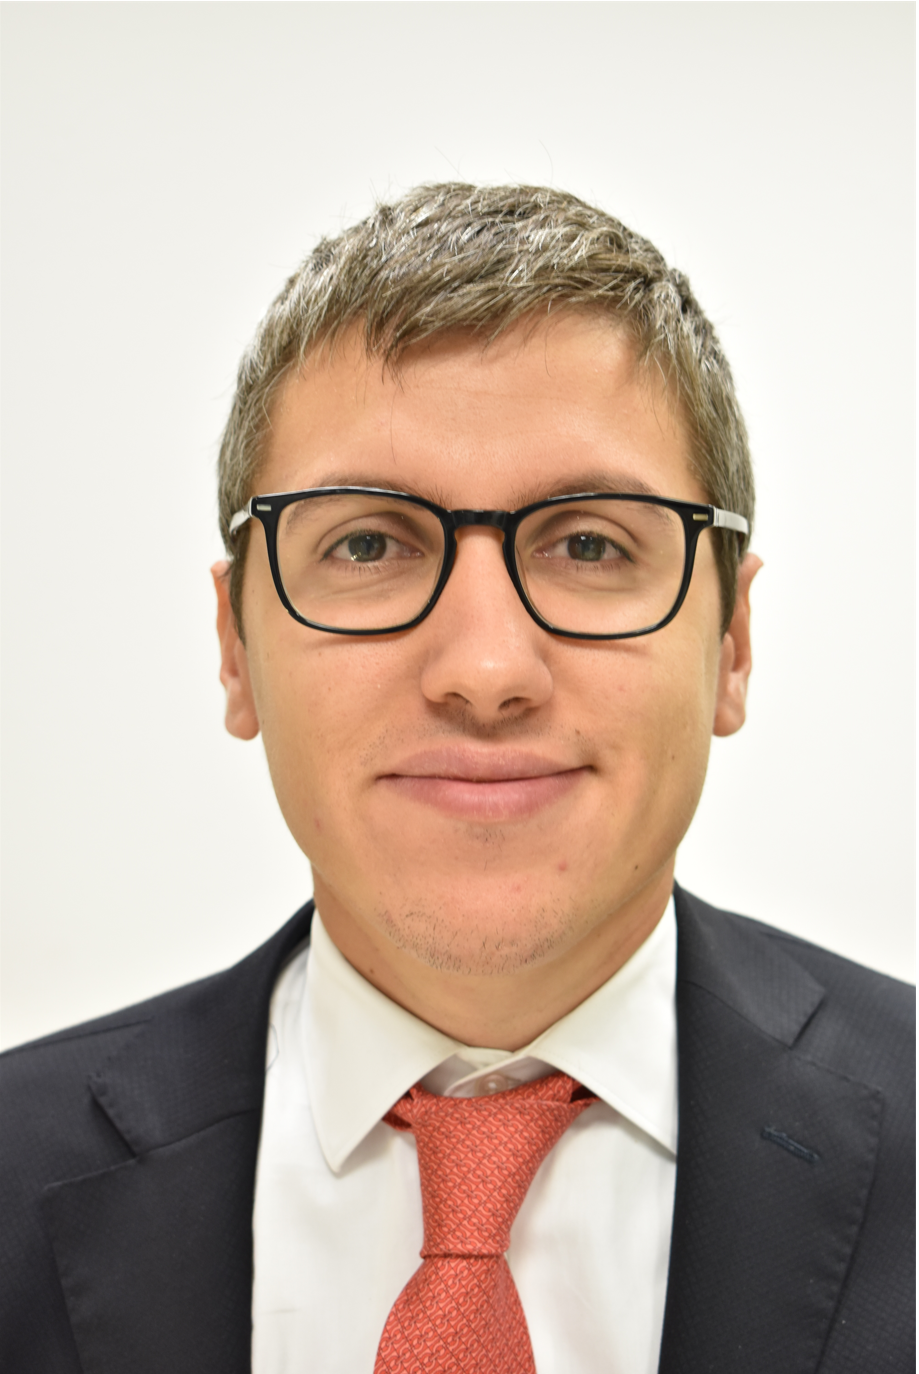
\includegraphics[height=6cm]{own_picture.png}};
\end{tikzpicture}
%----------------------------------------------------------------------------------------
%	NAME AND CONTACT INFORMATION SECTION
%----------------------------------------------------------------------------------------

\begin{cv}{\spacedallcaps{Davide Bossoli}}\vspace{1.5em} % Your name

\noindent\spacedlowsmallcaps{Personal Information}\vspace{0.5em} % Personal information heading

\NewEntry{}{\textit{Born in Italy,}}{21 August 1988} % Birthplace and date

\NewEntry{email}{\href{mailto:davidebossoli@libero.it}{davidebossoli@libero.it}} % Email address

%\NewEntry{website}{\href{http://www.johnsmith.com}{http://www.johnsmith.com}} % Personal website

\NewEntry{phone}{(M) +39 3465076072} %\ \ $\cdotp$\ \ (M) +1 (000) 111 1112} % Phone number(s)

\vspace{1em} % Extra white space between the personal information section and goal
$\;$
\\
$\;$


%----------------------------------------------------------------------------------------
%	WORK EXPERIENCE
%----------------------------------------------------------------------------------------

\noindent\spacedlowsmallcaps{Work Experience}\vspace{1em}

\NewEntry{2018 - Now}{\textsc{AXA Italy}}

\Description{\MarginText{Senior data scientist}I am currently working as senior data scientist at AXA Italy. 
My main activity is to develop and manage core-business Artificial Intelligence data applications end to end, from the design phase to the development / deployment / monitoring ones. During these projects I also supervise and mentor cross-functional teams of data scientists and machine learning engineers.
\newline
Each application is developed and deployed in a private AWS Cloud using for instance services for ETL tasks (Glue, EMR), machine learning (Sagemaker), serverless processing (Lambda) monitoring and exploration (Cloudwatch, Quicksight, Athena) and orchestration (Step).
For certain applications we also developed advanced Qlik Sense dashboards for data exploration or service monitoring.
\newline
I am also contributing to the development of data science frameworks for MLops, experiments tracking / reproducibility and training/serving data pipelines.
\newline
So far I had the opportunity to work mainly on hybrid deterministic / machine learning data applications.
}

\NewEntry{2016 - 2018}{\textsc{McKinsey Italy}}

\Description{\MarginText{AI consultant}I helped developing AI prototypes for different clients, use-cases and industries such as banking, insurance, real estate, chemical, semiconductors and pharma.
Some of the projects I worked on were abroad, mainly UK and France.
\newline
I had the opportunity to work mainly on machine-learning prototypes.
}

%------------------------------------------------

\NewEntry{2013, 2014-2016}{\textsc{Karolinska Institutet, Biostatistics department}}

\Description{\MarginText{Visiting researcher}During my two periods at Karolinska Institute I worked on my master and Phd thesis, as well as holding statistical labs/seminars and practice as statistical consultant.
}

%------------------------------------------------

\NewEntry{2011 - 2012}{\textsc{Municipality of Bologna}}

\Description{\MarginText{Biostatistician}At the Municipality of Bologna I did an internship where I learned the basics of SAS and worked with epidemiological data from the region of Emilia-Romagna. Most of my work was related to studying the association between respiratory mortality and some pollutants such as ozone, particulate matter and nitrogen dioxite.}
$\;$
\\
$\;$
%------------------------------------------------

\vspace{5em} % Extra space between major sections

%----------------------------------------------------------------------------------------
%	EDUCATION
%----------------------------------------------------------------------------------------

\spacedlowsmallcaps{Education}\vspace{1em}

\NewEntry{2013 - 2016}{University of Padova}

\Description{\MarginText{Phd in Statistics}%\ \ $\cdotp$\ \ \textit{First Class Honours}\ \ $\cdotp$\ \ School: Business and Administration
\newline
In the first year I took advanced theoretical statistical courses.
During the other two years I worked on my PhD thesis, mostly at the Biostatistics Department of Karolinska Institutet; one of the algorithms that I developed during my thesis was also published in the journal Biostatistics.
\newline
Thesis: \textit{Extensions of marginal quantile regression to the analysis of dependent data}
\href{http://paduaresearch.cab.unipd.it/10008/}{Link to the thesis}
\newline}

\NewEntry{2011-2013}{University of Bologna}

\Description{\MarginText{Master of Statistics}Grade: 110/110 cum laude%\ \ $\cdotp$\ \ \textit{First Class Honours}\ \ $\cdotp$\ \ School: Business and Administration
\newline 
This degree focused heavily on statistical methodology and its application within the biomedical field. The main topics covered are parametric and non parametric inference, multilevel and generalized linear models, quantile regression, parametric and semiparametric survival analysis, non-parametric time series analysis.
\newline
Thesis: \textit{Logistic Quantile Mixed Models - an application to health condition data}
$\;$
\\
$\;$
\\
$\;$
%\newline
%Description: This thesis explored an extention of quantile regression, and was used to study the association between %perceived health status and a set of covariates.\newline
%Advisors: Prof.~Rossella \textsc{Miglio} \& Prof.~Matteo \textsc{Bottai}
%\newline
%\newline
\newline}


%------------------------------------------------

\NewEntry{2008-2011}{University of Bologna}

\Description{\MarginText{Bachelor of Statistics}Grade: 110/110 cum laude %\ \ $\cdotp$\ \ \textit{Commerce Specialization}\ \ $\cdotp$\ \ School: Business and Administration
\newline
Description: Most of this degree was related to the application of statistical methods for economics and business.
Some of the topics covered include structural equation modeling, principal component analysis, parametric time series and econometrics.
\newline
Thesis: \textit{Statistical models for the evaluation of competences}
%\newline
%\newline

%Description: After a brief introduction to Item Response Theory, we applied this methodology to study the performances of italian %students in a standardized mathematical test.
%\newline
%Advisors: Prof.~Stefania \textsc{Mignani} \& Asc. Prof.~Mariagiulia \textsc{Matteucci}


}

%------------------------------------------------

\vspace{1em} % Extra space between major sections

%----------------------------------------------------------------------------------------
%	PUBLICATIONS
%----------------------------------------------------------------------------------------

\spacedlowsmallcaps{Publications}\vspace{1em}

\NewEntry{October 2018}{Marginal quantile regression for dependent data with a working odds-ratio matrix}

\Description{\MarginText{Biostatistics journal}This paper contains part of my PhD work and focused on the extension of quantile regression for dependent data.
\newline
Authors: Davide \textsc{Bossoli}, ~Matteo \textsc{Bottai}
\newline
\href{https://academic.oup.com/biostatistics/article/19/4/529/4585737}{Link to the paper}

}

%------------------------------------------------

%\NewEntry{Sept. 2012}{Publication Title}

%\Description{\MarginText{Full Journal Name}Lorem ipsum dolor sit amet, consectetur adipiscing elit. Ut nisl tellus, sodales non %pulvinar in, adipiscing sit amet purus. Suspendisse sed facilisis diam. Sed ornare sem nec justo adipiscing nec venenatis lectus %commodo. Mauris non neque ligula. Pellentesque sed quam eu felis iaculis iaculis ac a leo. Suspendisse neque neque, placerat id %adipiscing et, elementum eu sem.\\ Authors: John \textsc{Smith}, ~James \textsc{Smith}}

%------------------------------------------------

\vspace{1em} % Extra space between major sections

%----------------------------------------------------------------------------------------
%	COMPUTER SKILLS
%----------------------------------------------------------------------------------------

\spacedlowsmallcaps{Advanced analytics use-cases and industries}\vspace{1em}

\Description{$\cdotp$ \textbf{Pricing} (insurance, real-estate)
\newline
$\cdotp$ \textbf{Black-boxes telematics scoring} (insurance)
\newline
$\cdotp$ \textbf{Retention} (insurance)
\newline
$\cdotp$ \textbf{Predictive maintenance} (semiconductors)
\newline
$\cdotp$ \textbf{Customer segmentation} (banking)
\newline
$\cdotp$ \textbf{Process automation} (insurance)
\newline
$\cdotp$ \textbf{Process optimization} (chemicals, pharma, payments)
}

\spacedlowsmallcaps{Cloud services and technologies}\vspace{1em}

\Description{\MarginText{Basic}\textsc{AWS IAM}, \textsc{AWS Cloudwatch}, \textsc{AWS Quicksight}, \textsc{AWS API Gateway}, \textsc{Docker}, \textsc{Terraform} }

\Description{\MarginText{Intermediate}\textsc{AWS Glue}, \textsc{AWS EMR}, \textsc{AWS Lambda}, \textsc{AWS Dynamodb}}

\Description{\MarginText{Advanced}\textsc{AWS Sagemaker}, \textsc{AWS Athena}}


\spacedlowsmallcaps{Software Languages and tools}\vspace{1em}

\Description{\MarginText{Basic}\textsc{stata}, \textsc{sas}, \textsc{spss}, \textsc{java}, \LaTeX}

\Description{\MarginText{Intermediate}\textsc{R}, \textsc{Qlik sense}, \textsc{Pyspark}}

\Description{\MarginText{Advanced}\textsc{Python}}


\spacedlowsmallcaps{Python libraries}\vspace{1em}

\Description{\textsc{pandas}, \textsc{numpy}, \textsc{multiprocessing}, \textsc{h2o},  \textsc{sklearn},  \textsc{matplotlib}}


\vspace{1em} % Extra space between major sections
%------------------------------------------------


%----------------------------------------------------------------------------------------
%	OTHER INFORMATION
%----------------------------------------------------------------------------------------

\spacedlowsmallcaps{Other Information}\vspace{1em}

\Description{\MarginText{Awards}2013\ \ $\cdotp$\ \ School of Statistics Graduate Scholarship}

%\vspace{-0.5em} % Negative vertical space to counteract the vertical space between every \Description command

%\Description{2010\ \ $\cdotp$\ \ Top Achiever Award -- Commerce}

%------------------------------------------------

%\vspace{1em}

%\Description{\MarginText{Communication Skills}2010\ \ $\cdotp$\ \ Oral Presentation at the California Business Conference}

%\vspace{-0.5em} % Negative vertical space to counteract the vertical space between every \Description command

%\Description{2009\ \ $\cdotp$\ \ Poster at the Annual Business Conference in Oregon}

%------------------------------------------------

\vspace{1em}

\newlength{\langbox} % Create a new length for the length of languages to keep them equally spaced
\settowidth{\langbox}{English} % Length equals the length of "English" - if you have a longer language in your list put it here

\Description{\MarginText{Languages}\parbox{\langbox}{\textsc{Italian}}\ \ $\cdotp$\ \ \ Mothertongue}

\vspace{-0.5em} % Negative vertical space to counteract the vertical space between every \Description command

\Description{\parbox{\langbox}{\textsc{English}}\ \ $\cdotp$\ \ \ Advanced}

\vspace{-0.5em} % Negative vertical space to counteract the vertical space between every \Description command

%\Description{\parbox{\langbox}{\textsc{Spanish}}\ \ $\cdotp$\ \ \ Basic (simple words and phrases only)}

\vspace{1em} % Negative vertical space to counteract the vertical space between every \Description command

%------------------------------------------------

\Description{\MarginText{Personal interests}Reading books\ \ $\cdotp$\ \ Watching motor sports\ \ $\cdotp$\ \ Hiking\ \ $\cdotp$\ \ Exploring the world}

%----------------------------------------------------------------------------------------

\end{cv}

\end{document}